\documentclass{beamer}
\usepackage{subfig}
\usepackage{amsmath}
\usepackage{bm}

\DeclareMathOperator*{\argmax}{arg\,max}
\DeclareMathOperator*{\argmin}{arg\,min}


\title{Linear Regression}
\author{Prof. Alessandro Lucantonio}
\institute{Aarhus University - Department of Mechanical and Production Engineering}
\date{?/?/2023}

\begin{document}
	
	\frame{\titlepage}
	
	\section{Linear regression with one variable}

	\begin{frame}
		\frametitle{Weight-Height example}
		Dataset: heights and weights of different people.
		
		Task: build a model that predict the height given the weight. 
		
		\begin{figure}
			\centering
			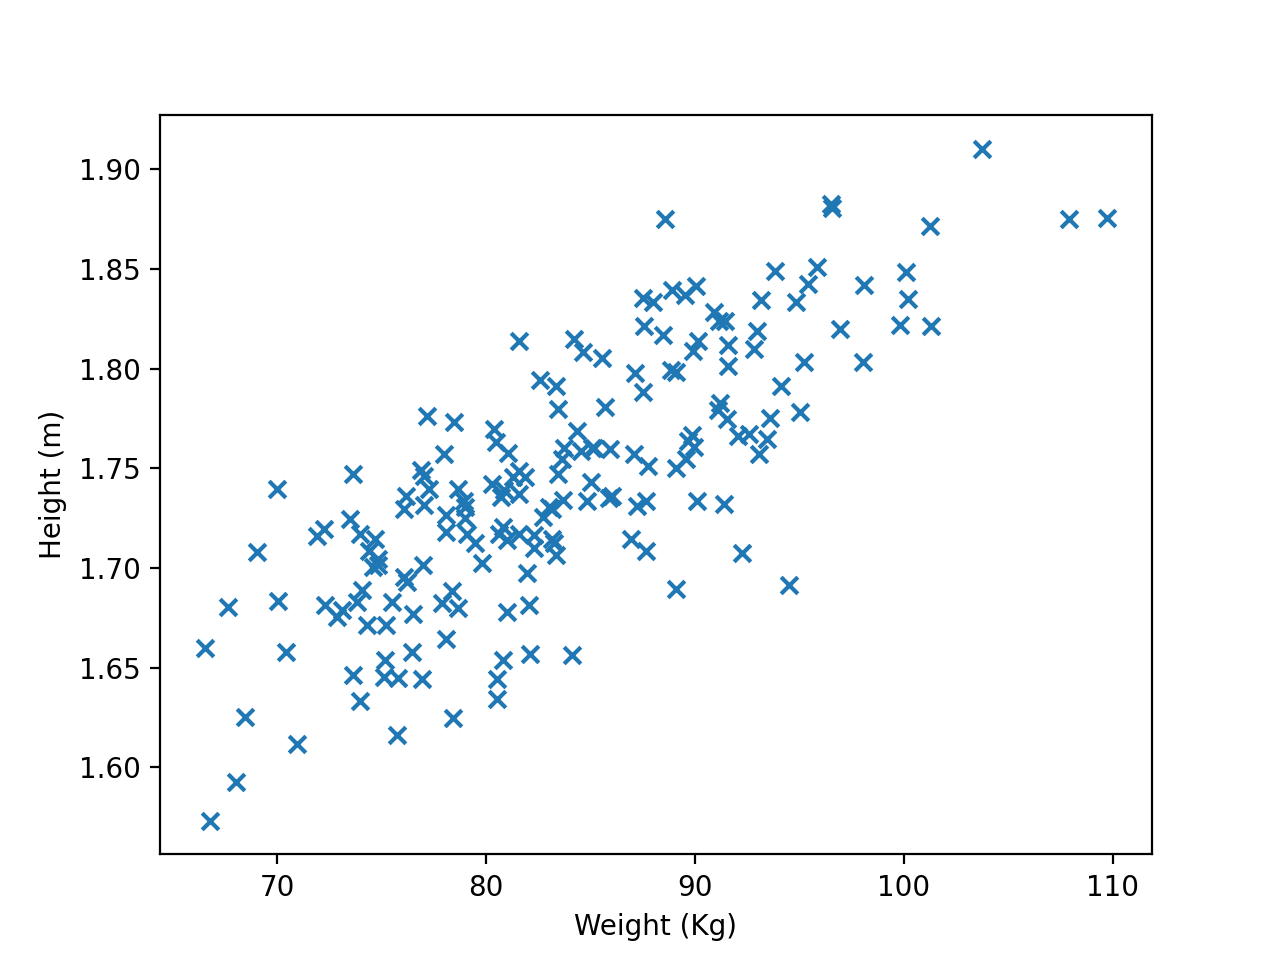
\includegraphics[scale=0.5]{images/linear_regression_data}
			\caption{Data plot}
		\end{figure}
	\end{frame}

	\begin{frame}
		\frametitle{A solution - Linear regression model}
		Some remarks on data.
		\begin{itemize}
			\item Regression problem (continuous output).
			\item Data with different order of magnitude.
		\end{itemize}
		A possible solution to this problem is represented by \textbf{linear regression} (LR).
		\begin{figure}
			\centering
			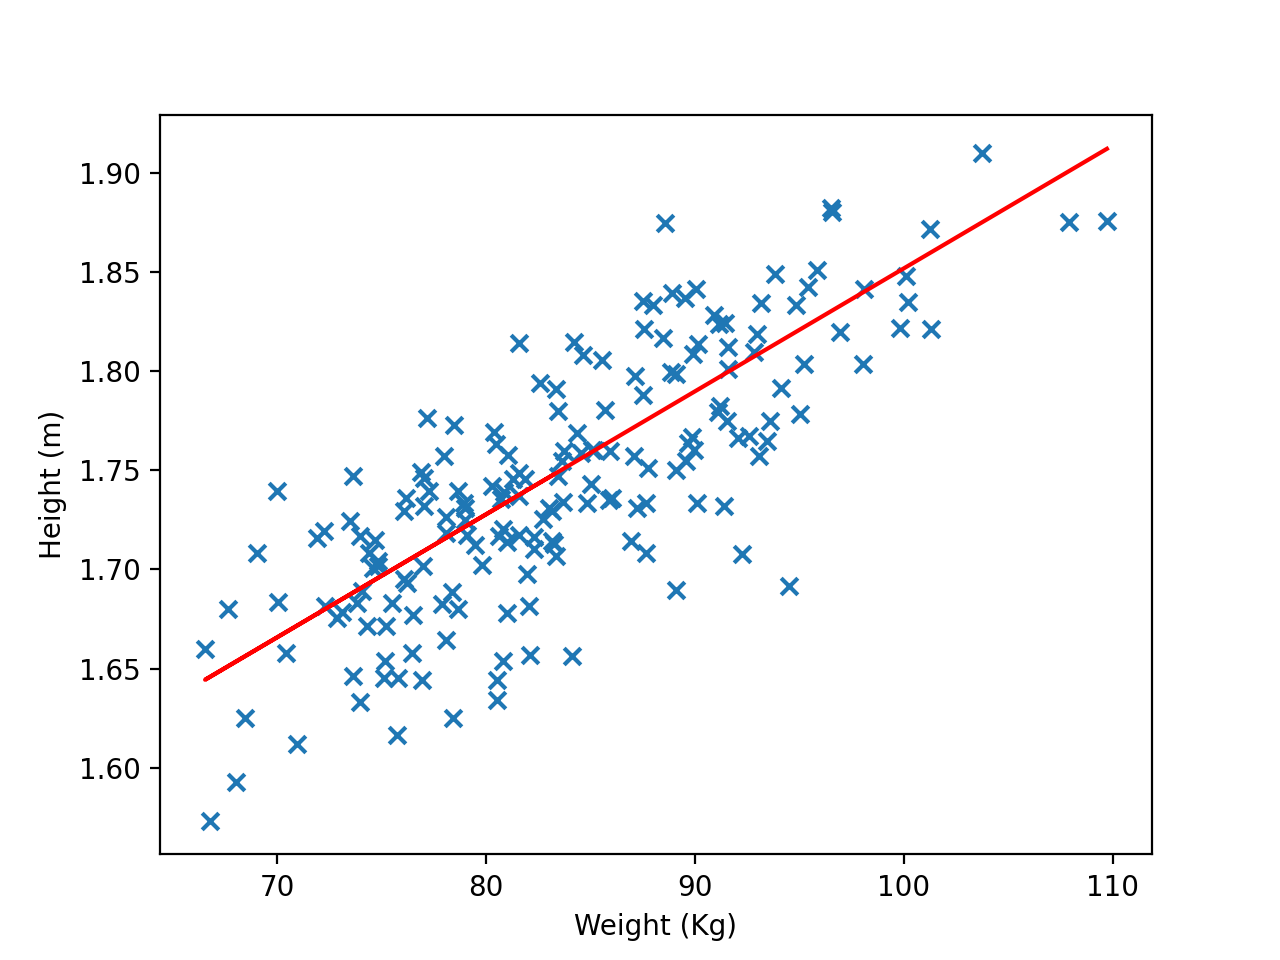
\includegraphics[scale=0.4]{images/linear_regression_fit}
			\caption{Trained model (in red)}
		\end{figure}
	\end{frame}

	\begin{frame}
		\frametitle{General ingredients}
		Notation:
		\begin{itemize}
			\item $x$: a data sample.
			\item $y$: the data target corresponding to $x$
			\item $N$: number of data.
		\end{itemize}
	
		\vspace{5 mm}
		
		Model/hypothesis: $h_{\bm{w}}(x) = w_1x + w_0$, where $\bm{w} = [w_0, w_1]$ is the vector of parameter that has to be learned.
		
		In our example, $x$ is the weight of a single sample and $h_{\bm{w}}(x)$ corresponds to the prediction of its height. 
		
		\vspace{5 mm}
		
		Usually the vector $\bm{w}$ is called \textbf{weights vector} and the set $\mathcal{H}:= \{h_{\bm{w}}| \bm{w} \in \mathbb{R}^2\}$ is called \textbf{hypothesis space}.
		
		\vspace{5 mm}
		
		How to learn $w$ from data?
		
	\end{frame}

	\begin{frame}
		\frametitle{Mean squared error (MSE)}
		
		
		Given a training sample $x_i$ and a model $h_{\bm{w}}$ we can predict the target computing $h_{\bm{w}}(x_i)$. To evaluate how good is the prediction we compute the error $(h_{\bm{w}}(x_i) - y_i)^2$.
		
		\vspace{5 mm}
		
		$(h_{\bm{w}}(x_i) - y_i)^2 \geq 0$ and $(h_{\bm{w}}(x_i) - y_i)^2 = 0$ if and only if $h_{\bm{w}}(x_i) = y_i$. The \textbf{mean squared error} (MSE) is:
		$$E({\bm{w}}) := \frac{1}{N} \sum_{i=1}^{N} (h_{\bm{w}}(x_i) - y_i)^2.$$
		
		To find the best model we minimize the training error, hence in this case the MSE.
		
		$$\bm{w} \in \argmin_{\tilde{\bm{w}} \in \mathbb{R}^2} E(\tilde{\bm{w}}).$$
		
	\end{frame}

	\begin{frame}
		\frametitle{$n$-dimensional LR}
		\textsl{Dataset samples}.
		
		Previous case: $x \in \mathbb{R}, y \in \mathbb{R}$.
		
		\vspace{1 mm}
		
		Now:  $\bm{x} \in \mathbb{R}^n, y \in \mathbb{R}$.
		
		Notation: $x^i_j$ is the $j$-th coordinate of the $i$-th sample.
		
		\vspace{5 mm}
		
		\textsl{Hypothesis}.
		
		Previous case: 
		\begin{equation*}
			h_{w}(x) = w_1x + w_0,
		\end{equation*}
		where $w = [w_0, w_1]$.
		
		\vspace{1 mm}
		
		Now: 
		\begin{align*}
			h_{\bm{w}}(\bm{x}) &= w_{n}x_n + w_{n-1}x_{n-1} + \dots + w_1 x_1 + w_0\\
			&= \sum_{i=0}^n w_i \tilde{x}_i = \bm{w}^T \tilde{\bm{x}},\\
		\end{align*}
		where $\bm{w} = [w_0, \dots, w_n]$ and $\tilde{\bm{x}} = [1, x_1, \dots, x_n]$.
		
	\end{frame}

	\begin{frame}
		\frametitle{n-dimensional LR}
		\textsl{MSE}.
		
		Previous case: 
		\begin{equation*}
			E(\bm{w}) = \frac{1}{N} \sum_{i=1}^{N} (h_{\bm{w}}(x_i) - y_i)^2.
		\end{equation*}
		
		\vspace{1 mm}
		
		Now: 
		\begin{align*}
			E(\bm{w}) &= \frac{1}{N} \sum_{i=1}^{N} (h_w(\bm{x}^i) - y^i)^2\\
			&= \frac{1}{N} (\mathsf{X} \bm{w} - \bm{y})^T (\mathsf{X}\bm{w} - \bm{y})\\
			&= \frac{1}{N} ||\mathsf{X}\bm{w} - \bm{y}||^2
		\end{align*}
		
		where
		\begin{equation*}
			\mathsf{X} := \begin{bmatrix}
				\tilde{\bm{x}}^1\\
				\vdots\\
				\tilde{\bm{x}}^N 
			\end{bmatrix} \quad \bm{y} = \begin{bmatrix}
			y_1 \\
			\vdots\\
			y_N
		\end{bmatrix}.
		\end{equation*}
	\end{frame}

	\begin{frame}
		\frametitle{Spot the minimum - Gradient descent}
		How to find $\bm{w} \in \argmin_{\tilde{\bm{w}} \in \mathbb{R}^2} E(\tilde{\bm{w}})$?
		
		\vspace{5mm}
		
		Main idea: the gradient of a scalar field represent geometrically the direction with maximum slope. Hence, following the opposite direction of the gradient lead us to get closer to the minimum of the function.
		
		\vspace{5mm}
		
		Formally:
		\begin{itemize}
			\item Start with a random $\bm{w}^0$.
			\item For $j \geq 0$, update $\bm{w}^{j+1} := \bm{w}^{j} + \bm{d}^j$, where $\bm{d}^j$ is such that
			\begin{equation*}
				E(\bm{w}^{j+1}) \leq E(\bm{w}^j) 
			\end{equation*}
		\end{itemize}
		Gradient descent: $\bm{d}^j = - \alpha \nabla E(\bm{w}^j)$. $\alpha$ is called \textbf{learning rate}.
	\end{frame}

	\begin{frame}
		\frametitle{Gradient descent - 3D visualization}
		\begin{figure}
			\centering
			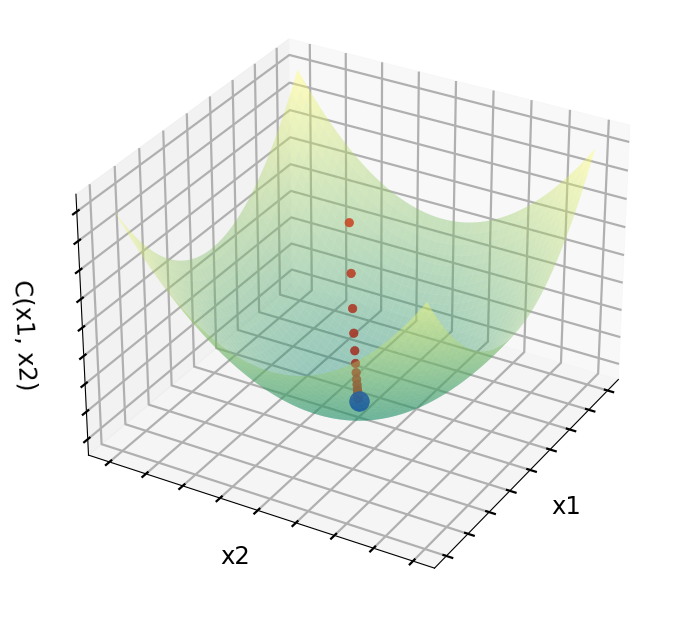
\includegraphics[scale=0.4]{images/gradient_descent_3D}
			\caption{In blue the global minimum, in red the iteration points.}
		\end{figure}
	\end{frame}

	\begin{frame}
		\frametitle{Gradient descent - 2D visualization}
		\begin{figure}
			\centering
			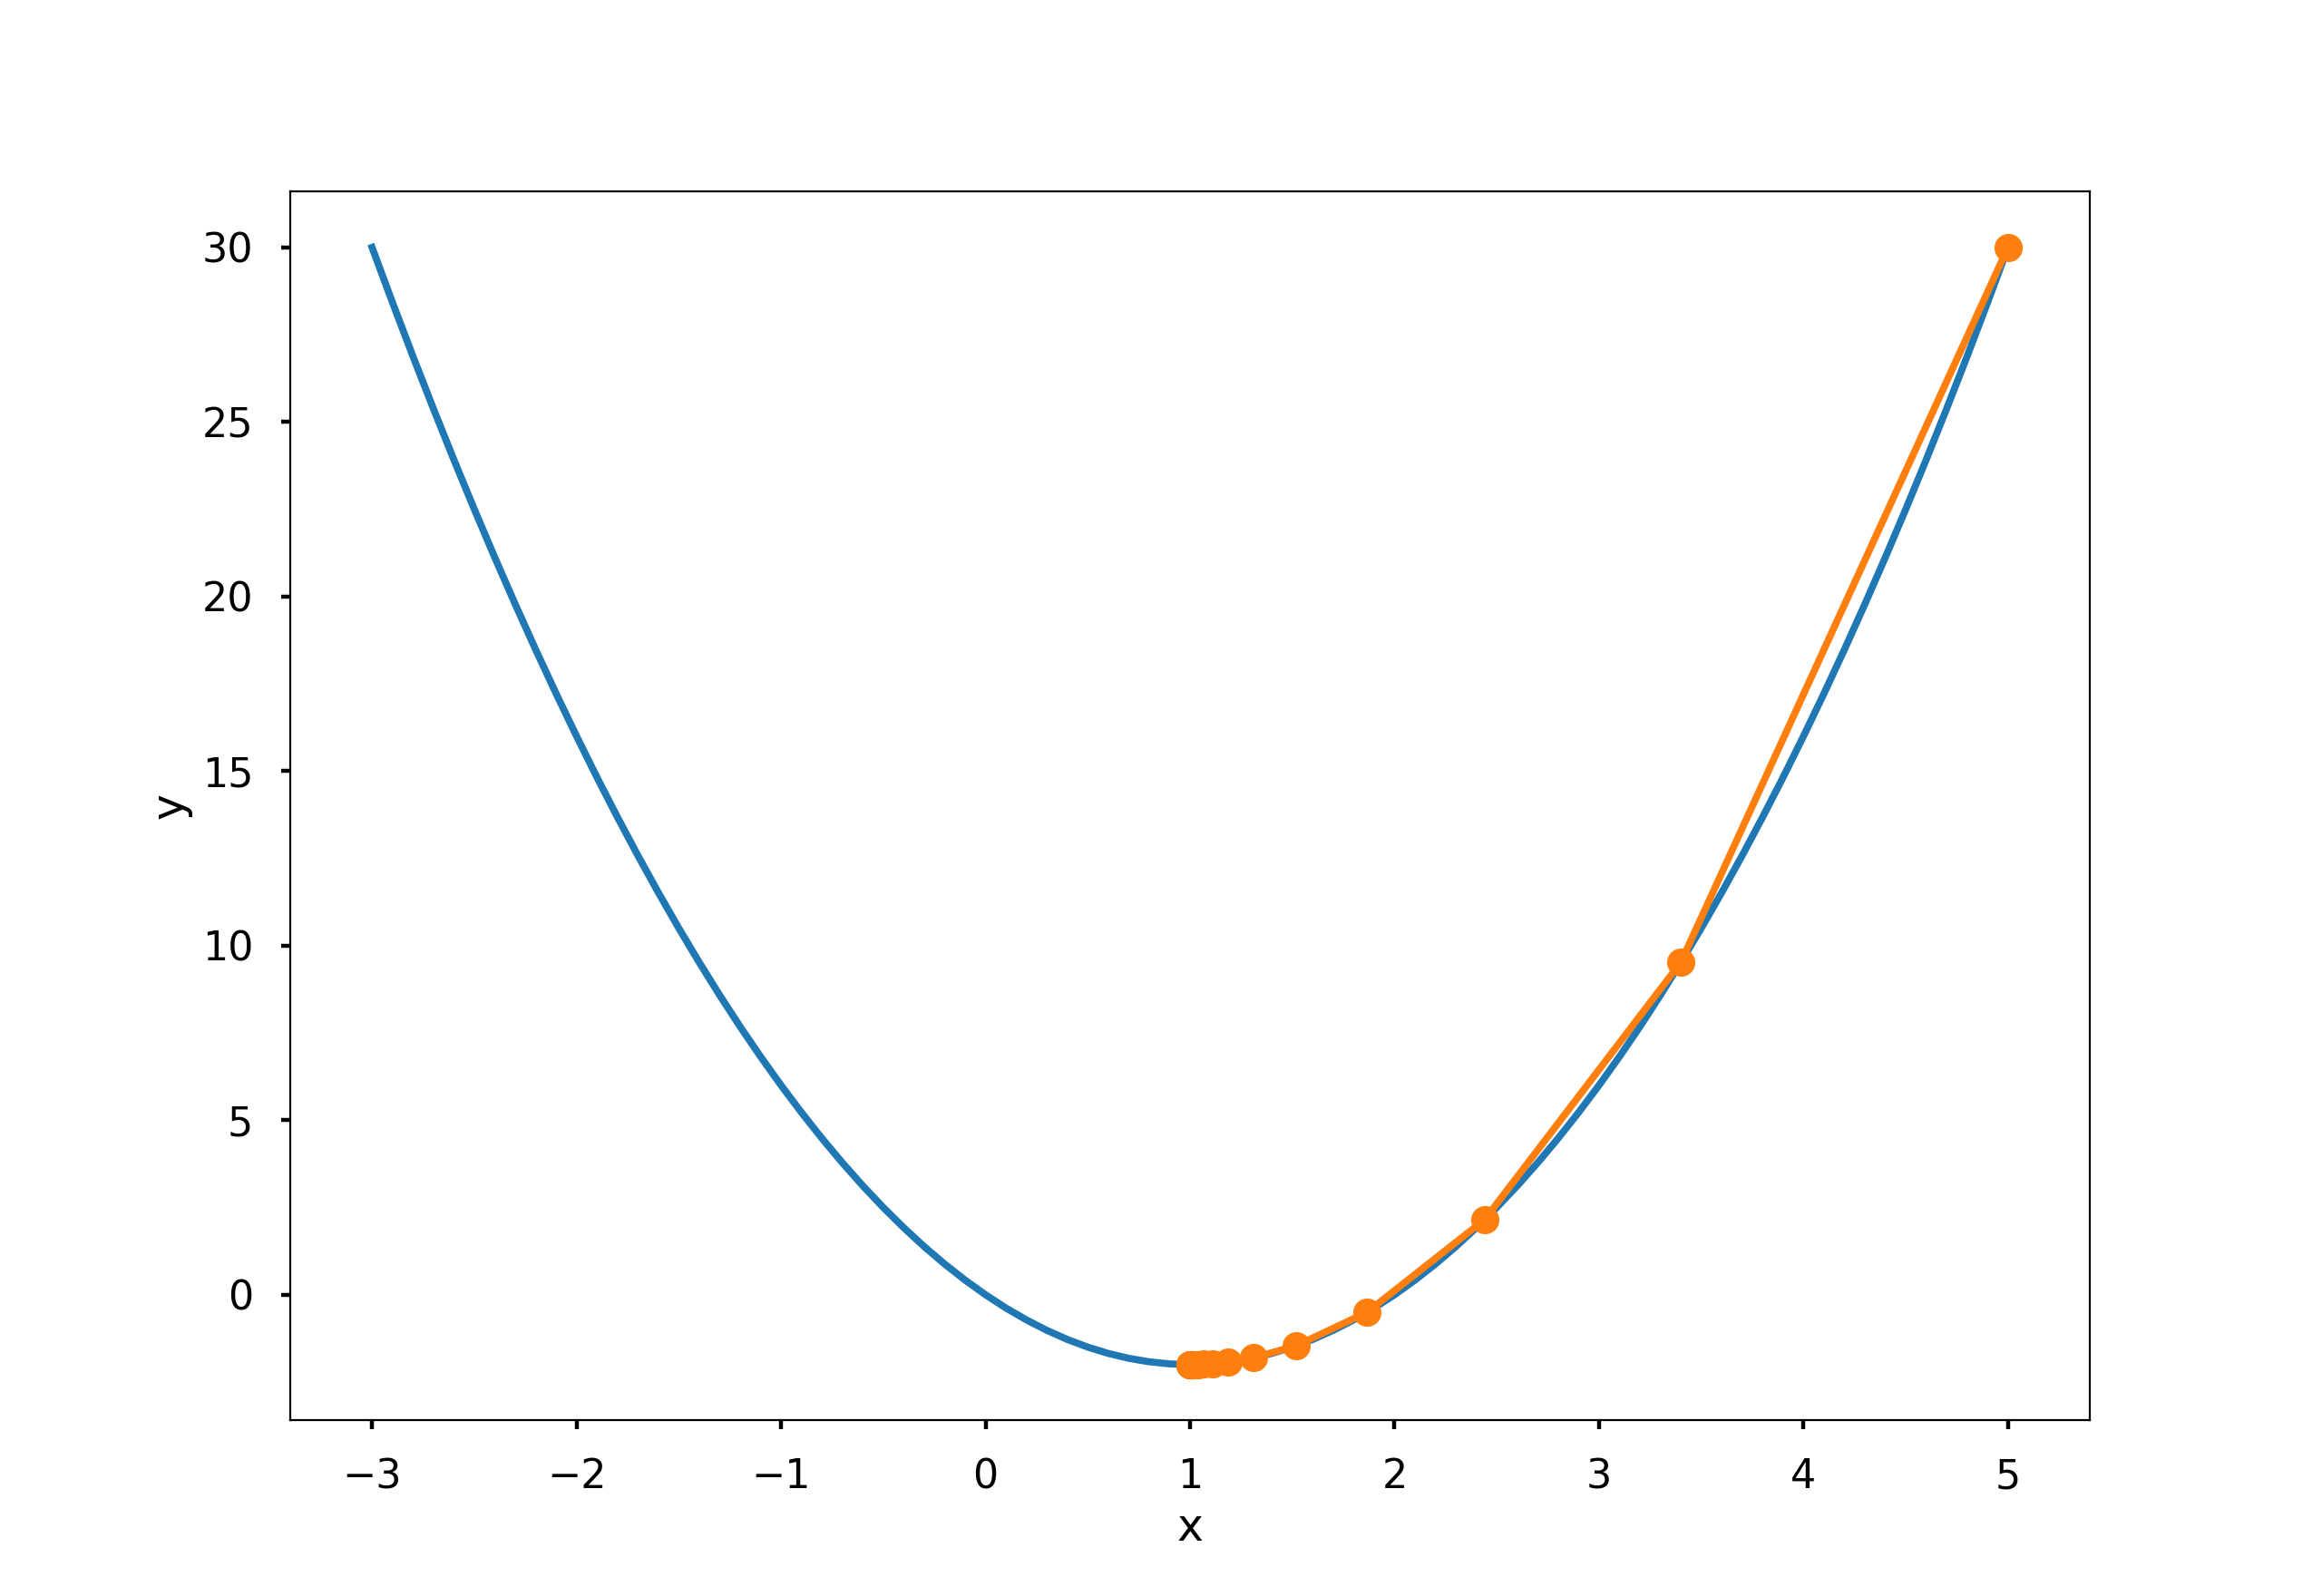
\includegraphics[scale=0.3]{images/gradient_descent_1}
			\caption{Learning rate = 0.1}
		\end{figure}
	\end{frame}

	\begin{frame}
		\frametitle{Gradient descent - 2D visualization}
		\begin{figure}
			\centering
			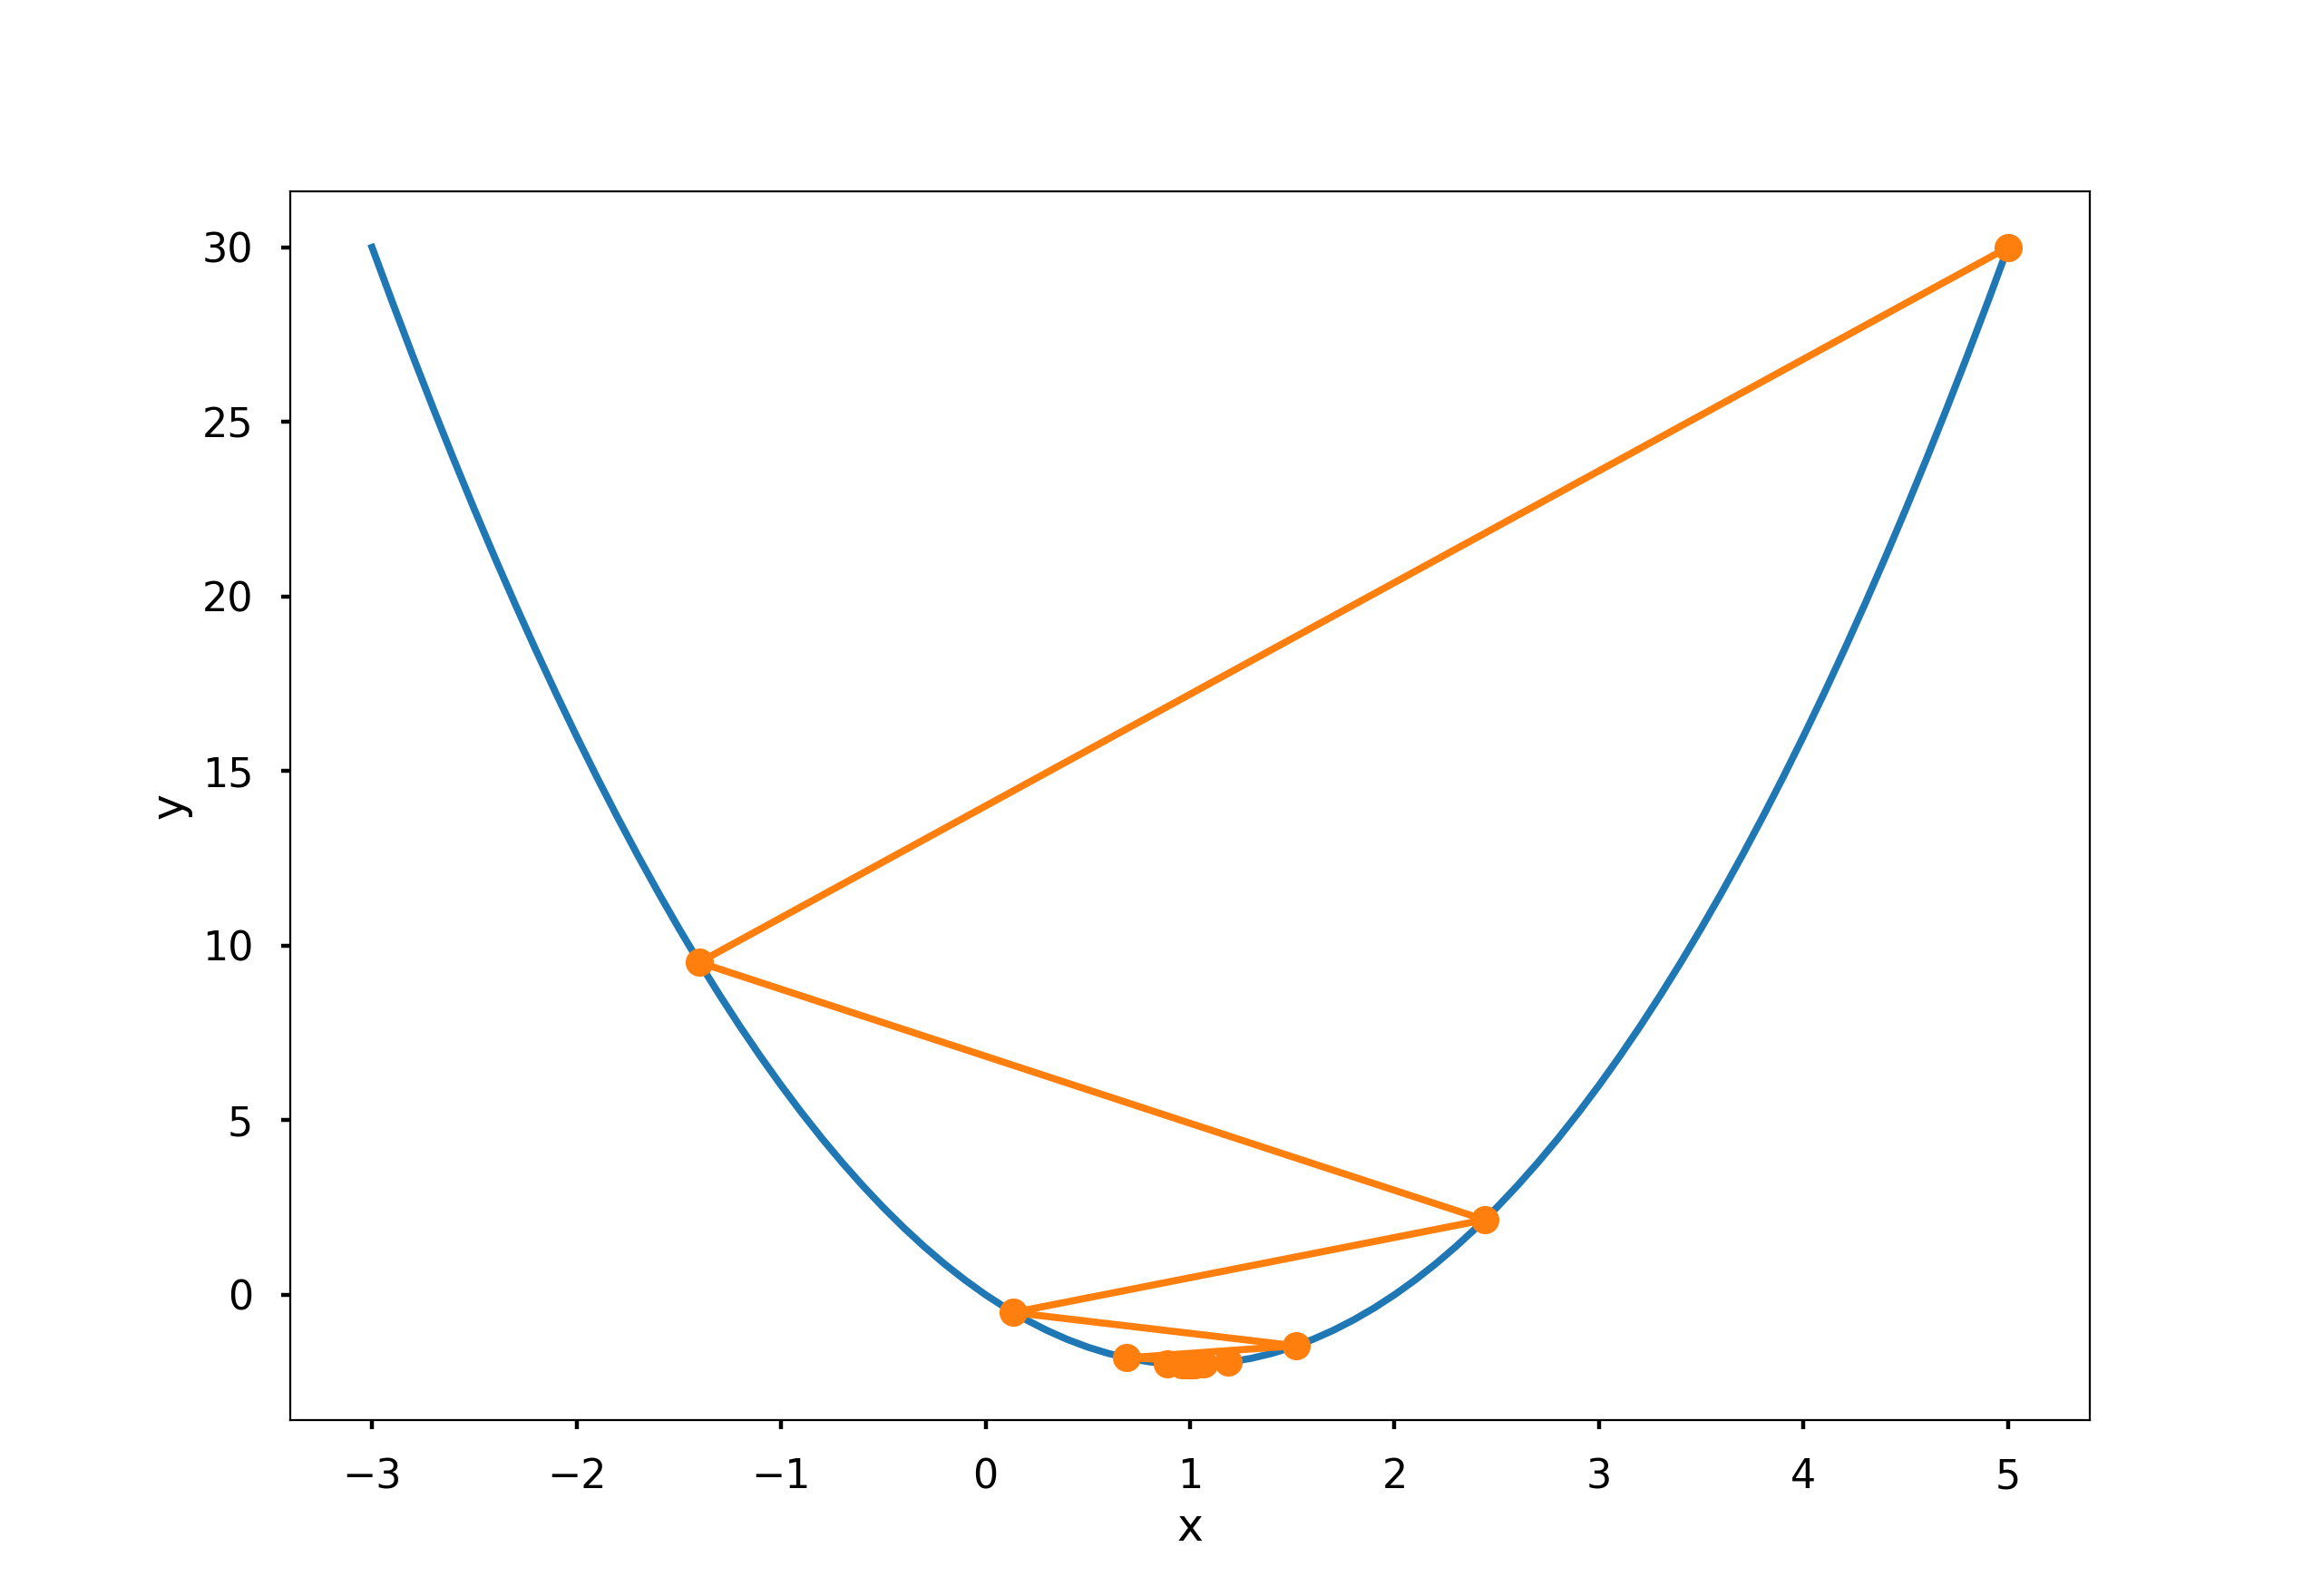
\includegraphics[scale=0.3]{images/gradient_descent_2}
			\caption{Learning rate = 0.4}
		\end{figure}
	\end{frame}

	\begin{frame}
		\frametitle{Gradient descent - 2D visualization}
		\begin{figure}
			\centering
			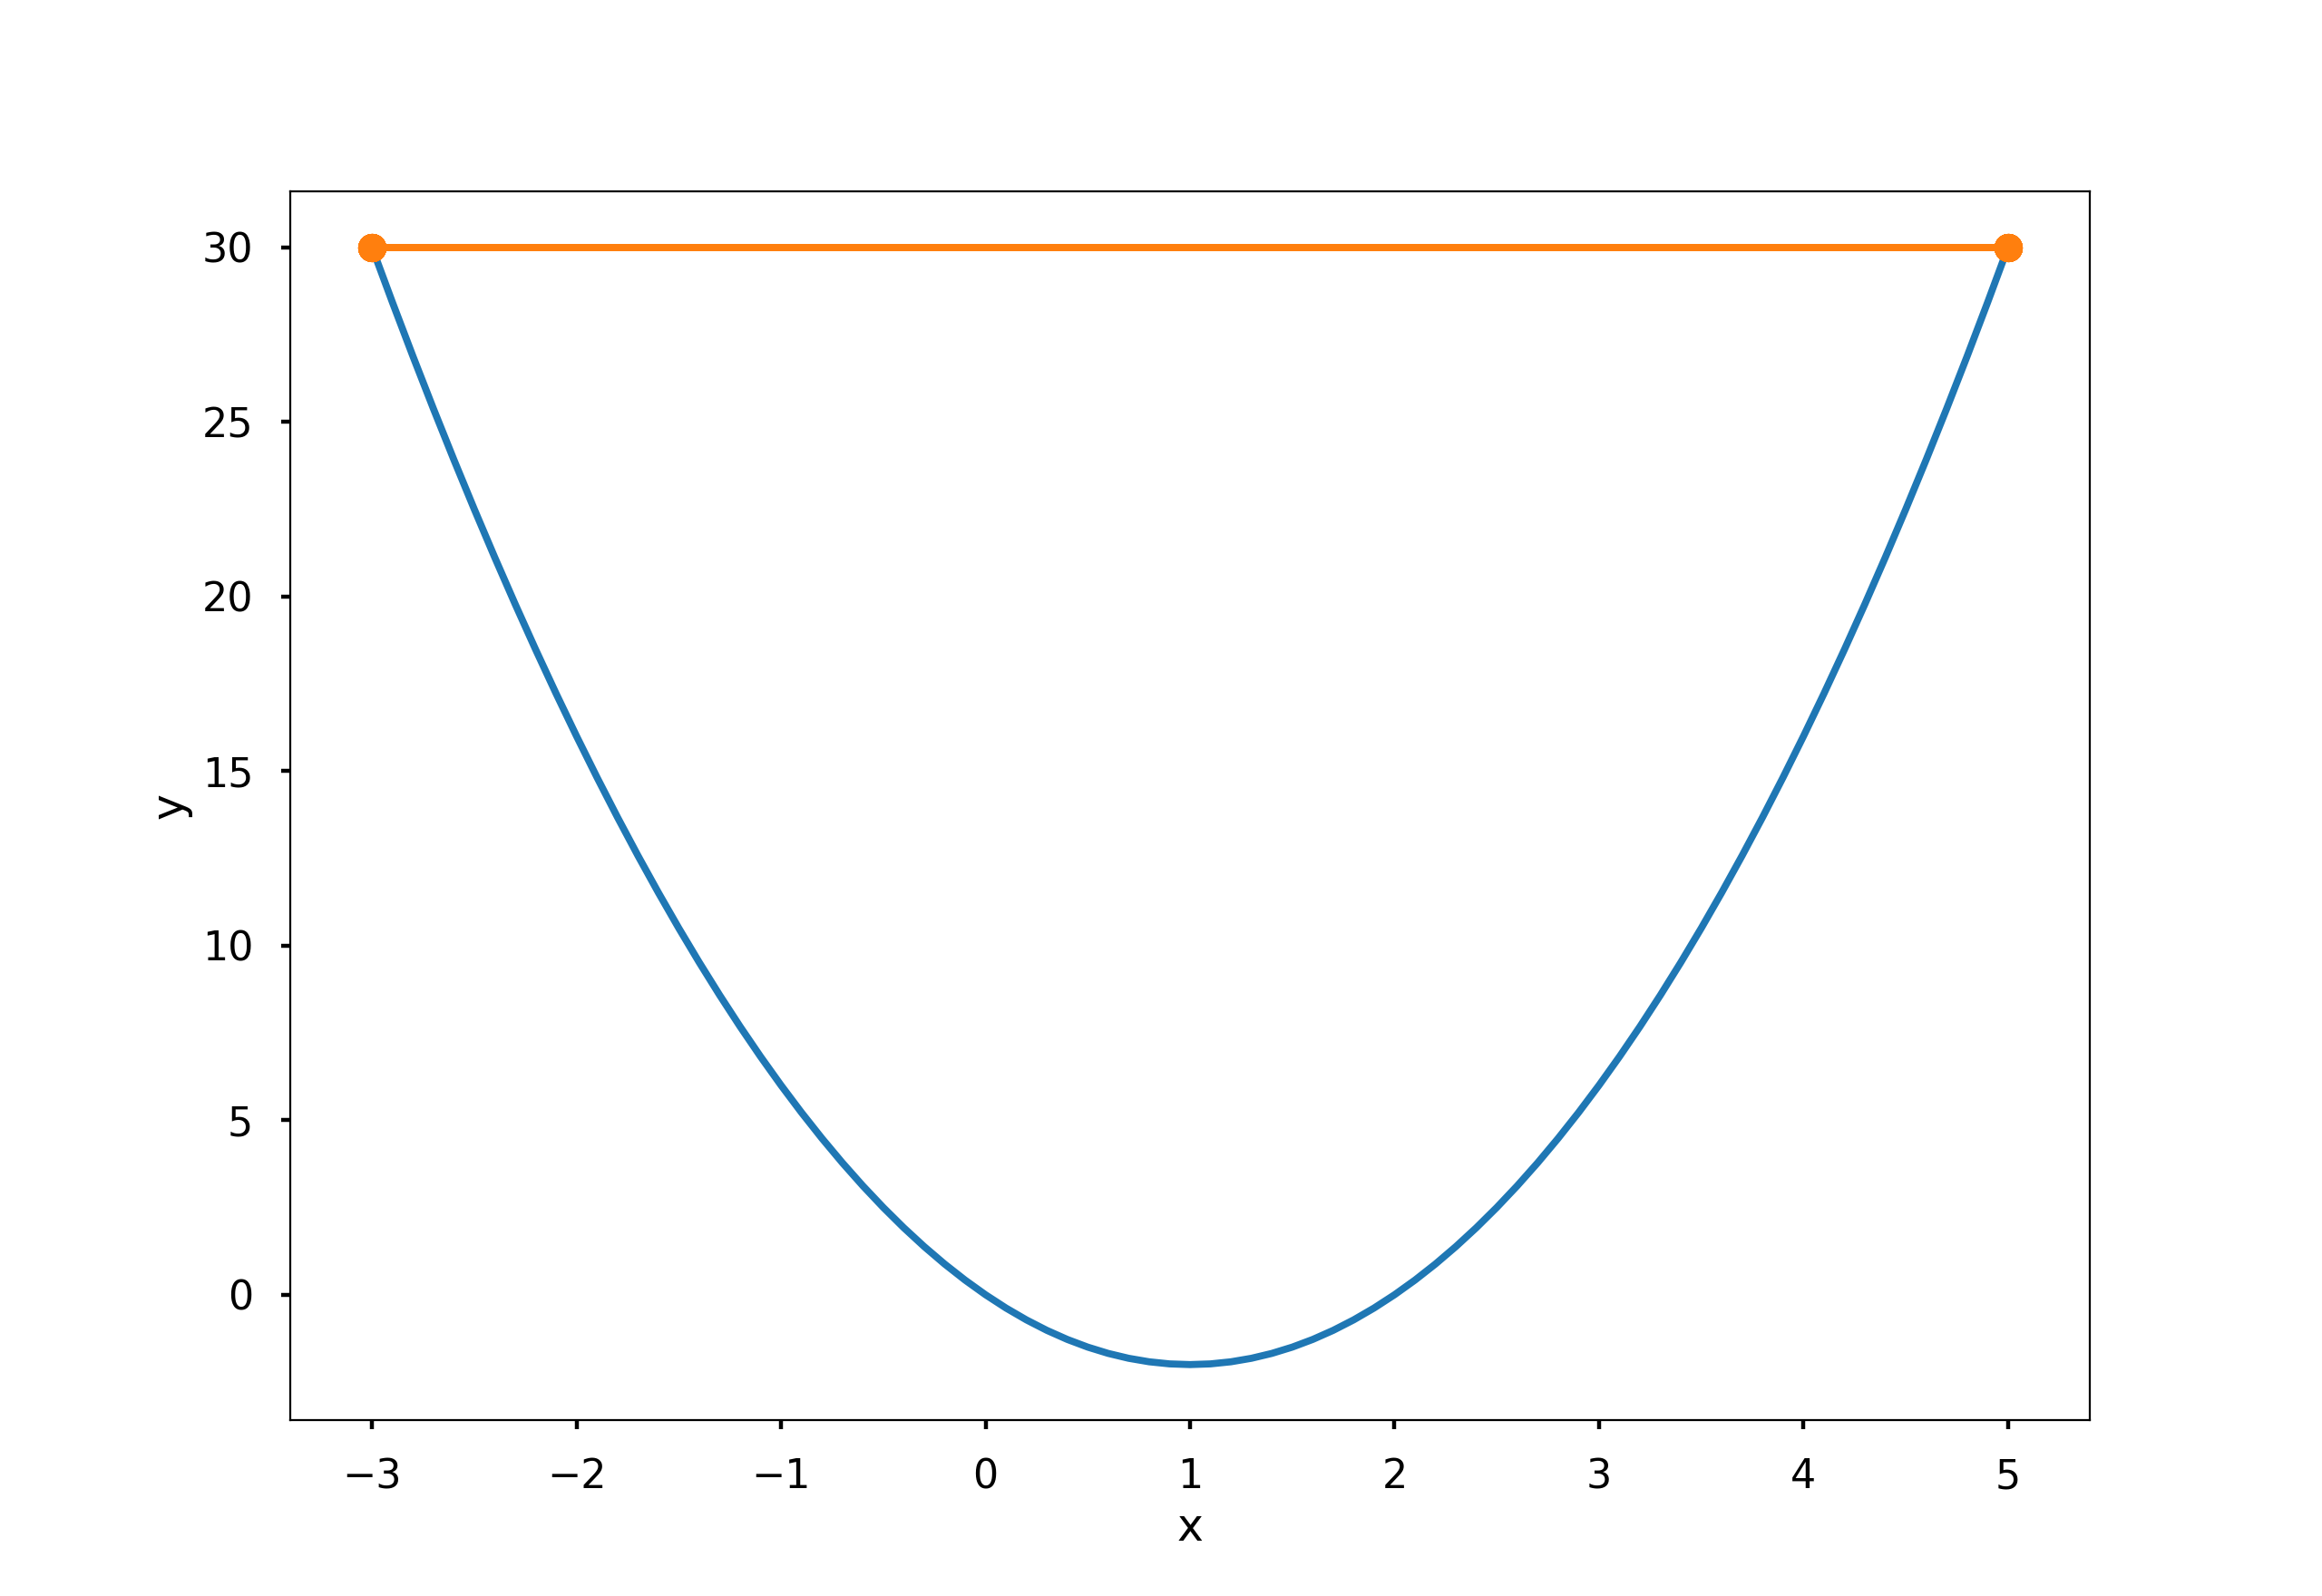
\includegraphics[scale=0.3]{images/gradient_descent_3}
			\caption{Learning rate = 0.5}
		\end{figure}
	\end{frame}

	\begin{frame}
		\frametitle{Batch, SGD and Mini-Batch}
		Notation: $E(\bm{w}) = 1/N \sum_{i=1}^N E_i(\bm{w})$
		
		\vspace{5mm}
		
		\textbf{Batch}
		\begin{itemize}
			\item Start with a random $\bm{w}^0$.
			\item For $j \geq 0$, update $\bm{w}^{j+1} := \bm{w}^{j} - \alpha \nabla E(\bm{w}^j)$.
		\end{itemize}
		
		\textbf{Stochastic Gradient Descent} (SGD or online)
		\begin{itemize}
			\item Start with a random $\bm{w}^0$.
			\item For $j \geq 0$ and for each pattern $1\leq i \leq N$ update $\bm{w}^{j+1} := \bm{w}^{j} - \alpha \nabla E_i(\bm{w}^j)$.
		\end{itemize}
	
		\textbf{Mini-Batch}. Fix an integer $1 \leq \text{mb} \leq N$(mini-batch size).
		\begin{itemize}
			\item Start with a random $\bm{w}^0$.
			\item For $j \geq 0$ and for each pattern $0 \leq i < \frac{N}{\text{mb}}$ update
			\begin{equation*}
				\bm{w}^{j+1} := \bm{w}^{j} - \alpha \nabla \sum_{k=i\cdot\text{mb} + 1}^{(i+1)\cdot\text{mb}}E_k(\bm{w}^j)
			\end{equation*}
		\end{itemize}
		
	\end{frame}

	\begin{frame}
		\frametitle{Tips and Tricks - How to choose?}
		\begin{itemize}
			\item Batch: usually more stable and provide a more accurate estimation of the gradient, but very slow.
			\item SGD: very fast, stochastic approximation of the gradient implies possible instability (Zig-zag effect)
			\item Mini-Batch: a trade-off (parallelism available).
		\end{itemize}
		\begin{figure}
			\centering
			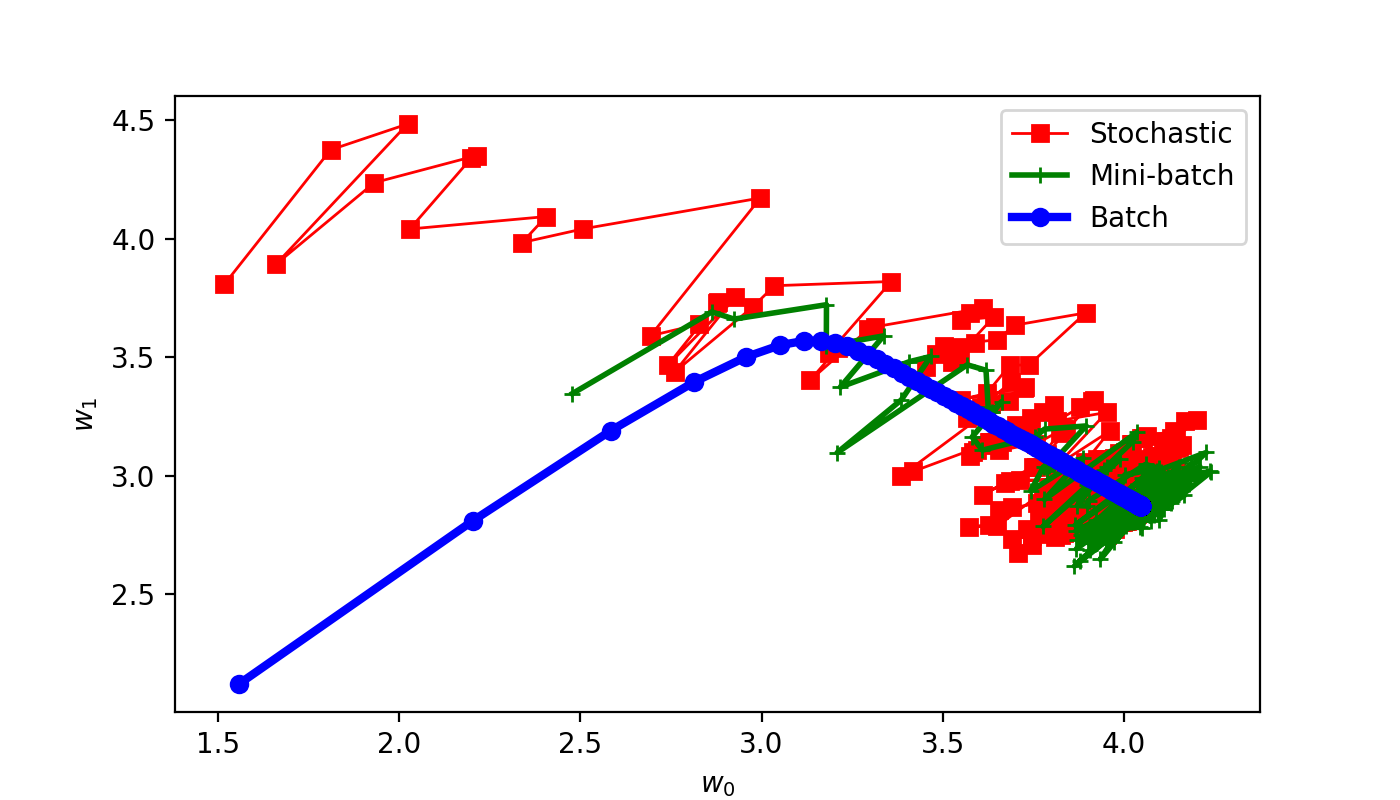
\includegraphics[scale=0.4]{images/gd_mb_sgd}
			\caption{Batch vs SGD vs Mini-batch}
		\end{figure}
	
	\end{frame}

	\begin{frame}
		\frametitle{Gradient descent and normal equation for LR}
		We have $E(\bm{w}) = \frac{1}{N} ||\mathsf{X}\bm{w} - \bm{y}||^2$, hence
		\begin{equation*}
			\nabla E(\bm{w}) = \frac{1}{N} \nabla (||\mathsf{X}\bm{w} - \bm{y}||^2) = \frac{2}{N}\mathsf{X}^T(\mathsf{X}\bm{w} - \bm{y})
		\end{equation*}
	
	Normal equation ($\textcolor{red}{\iff}$ holds if $\mathsf{X}^T\mathsf{X}$ is invertible):
	\begin{align*}
		\nabla E(\bm{w}) = 0 &\iff \frac{2}{N}\mathsf{X}^T(\mathsf{X}\bm{w} - \bm{y}) = 0\\ 
		&\iff \mathsf{X}^T\mathsf{X}\bm{w} = \mathsf{X}^T\bm{y}\\
		& \textcolor{red}{\iff} \bm{w} = (\mathsf{X}^T\mathsf{X})^{-1}\mathsf{X}^T\bm{y}
	\end{align*}
	
	Gradient descent main iteration for LR:
	
	\begin{equation*}
		\bm{w}^{j+1} := \bm{w}^{j} - \frac{2\alpha}{N}\mathsf{X}^T(\mathsf{X}\bm{w}^j - \bm{y})
	\end{equation*}
	
		
	\end{frame}

	\begin{frame}
		\frametitle{Normal equation vs gradient descent}
		Normal equation:
		\begin{itemize}
			\item No hyperparameter (explicit solution).
			\item No need to iterate.
			\item $\mathcal{O}(n^3)$, hence slow when $n$ is large.
		\end{itemize}
	
		\vspace{5mm}
	
		Gradient descent:
		\begin{itemize}
			\item Need to choose the learning rate $\alpha$.
			\item Needs many iterations.
			\item $\mathcal{O}(kn^2)$, hence fast when $n$ is large.
		\end{itemize}
	\end{frame}

	\begin{frame}
		\frametitle{Tips and Tricks - Standardization}
		General (not only for LR): features must be on a similar scale!
		\begin{itemize}
			\item Speed up the convergence of gradient descent.
			\item Try to have (on average) $-1 \leq x^i \leq 1$.
		\end{itemize}
		Common techniques:
		\begin{itemize}
			\item \textbf{Feature scaling}. Compute the max $\bm{M}$ and the min $\bm{m}$ data value. Then normalize each feature as follows
			\begin{equation*}
				\bm{x}_{\text{norm}}^i = \frac{\bm{x}^i - \bm{m}}{\bm{M} - \bm{m}}
			\end{equation*} 
			\item \textbf{Mean normalization}. Compute mean $\mu$ and standard deviation $\sigma$ of the data. Then normalize each feature as follows
			\begin{equation*}
				\bm{x}_{\text{norm}}^i = \frac{\bm{x}^i -\bm{\mu}}{\bm{\sigma}} 
			\end{equation*}
		\end{itemize}
	\end{frame}

	\begin{frame}
		\frametitle{Tips and Tricks - Standardization}
		\begin{figure}
			\centering
			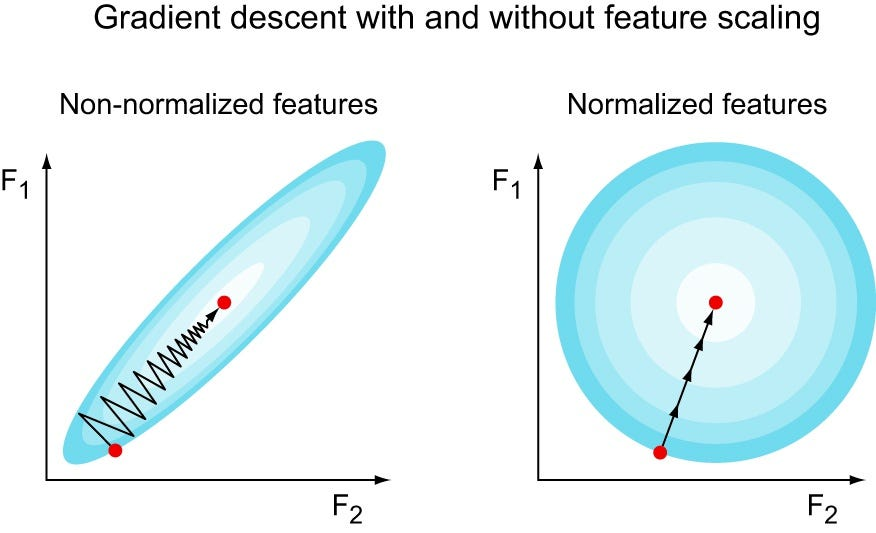
\includegraphics[scale=0.35]{images/feature-scaling}
		\end{figure}

		
	\end{frame}

	\begin{frame}
		\frametitle{Tips and Tricks - Invertibility of $\mathsf{X}^T\mathsf{X}$}
		What happens when $\mathsf{X}^T\mathsf{X}$ is not invertible?
		
		Invertibility of $\mathsf{X}^T\mathsf{X} =$ column of $X$ linearly independent (preprocessing information)
		
		\vspace{5mm}
		
		If a column is linearly dependent to the other then a feature is correlated with others (redundant feature).
		
		\vspace{5mm}
		
		Solution: discard that feature. The information carried by that feature is contained in some of the others. 
	\end{frame}

	\begin{frame}
		\frametitle{Polynomial regression (PR)}
		LR corresponds to linear hypothesis, i.e. of the form
		\begin{equation*}
			h_{\bm{w}}(\bm{x}) = \bm{w}^T \bm{x}
		\end{equation*}
		
		\vspace{5mm}
		
		PR corresponds to polynomial hypothesis, i.e. of the form
		\begin{equation*}
			h_{\bm{w}}(\bm{x}) = \sum_{j=0}^n w_j x^j_j.
		\end{equation*}
		
		\vspace{5mm}
		More in general: linear basis expansion (LBE)
		\begin{equation*}
			h_{\bm{w}}(\bm{x}) = \sum_{j=0}^n w_j \phi_j(\bm{x}),
		\end{equation*}
		where $\phi_j: \mathbb{R}^n \rightarrow \mathbb{R}$.
	\end{frame}

	\begin{frame}
		\frametitle{Underfitting and overfitting - main intuition}
		
		Imagine that you have to prepare an exam. 
		
		\vspace{5mm}
		
		Doing only a few exercises lead a poor perfomance both on homeworks and on the exam exercises. This is called \textsl{underfitting}: you have a bad performance on the exam because you did not trained enough.
		
		\vspace{5mm}
		
		Moreover, brutally memorize all the homework lead to a perfect score on homeworks (trivially) but probably a bad score on the exam exercises. This is called \textsl{overfitting}: you have a bad performance on the exam because you did not captured the true essence of your homework, you have also memorize their ''noise'' (homework pecularities).
	\end{frame}

	\begin{frame}
		\frametitle{Underfitting and overfitting - another example}
		\begin{figure}
			\centering
			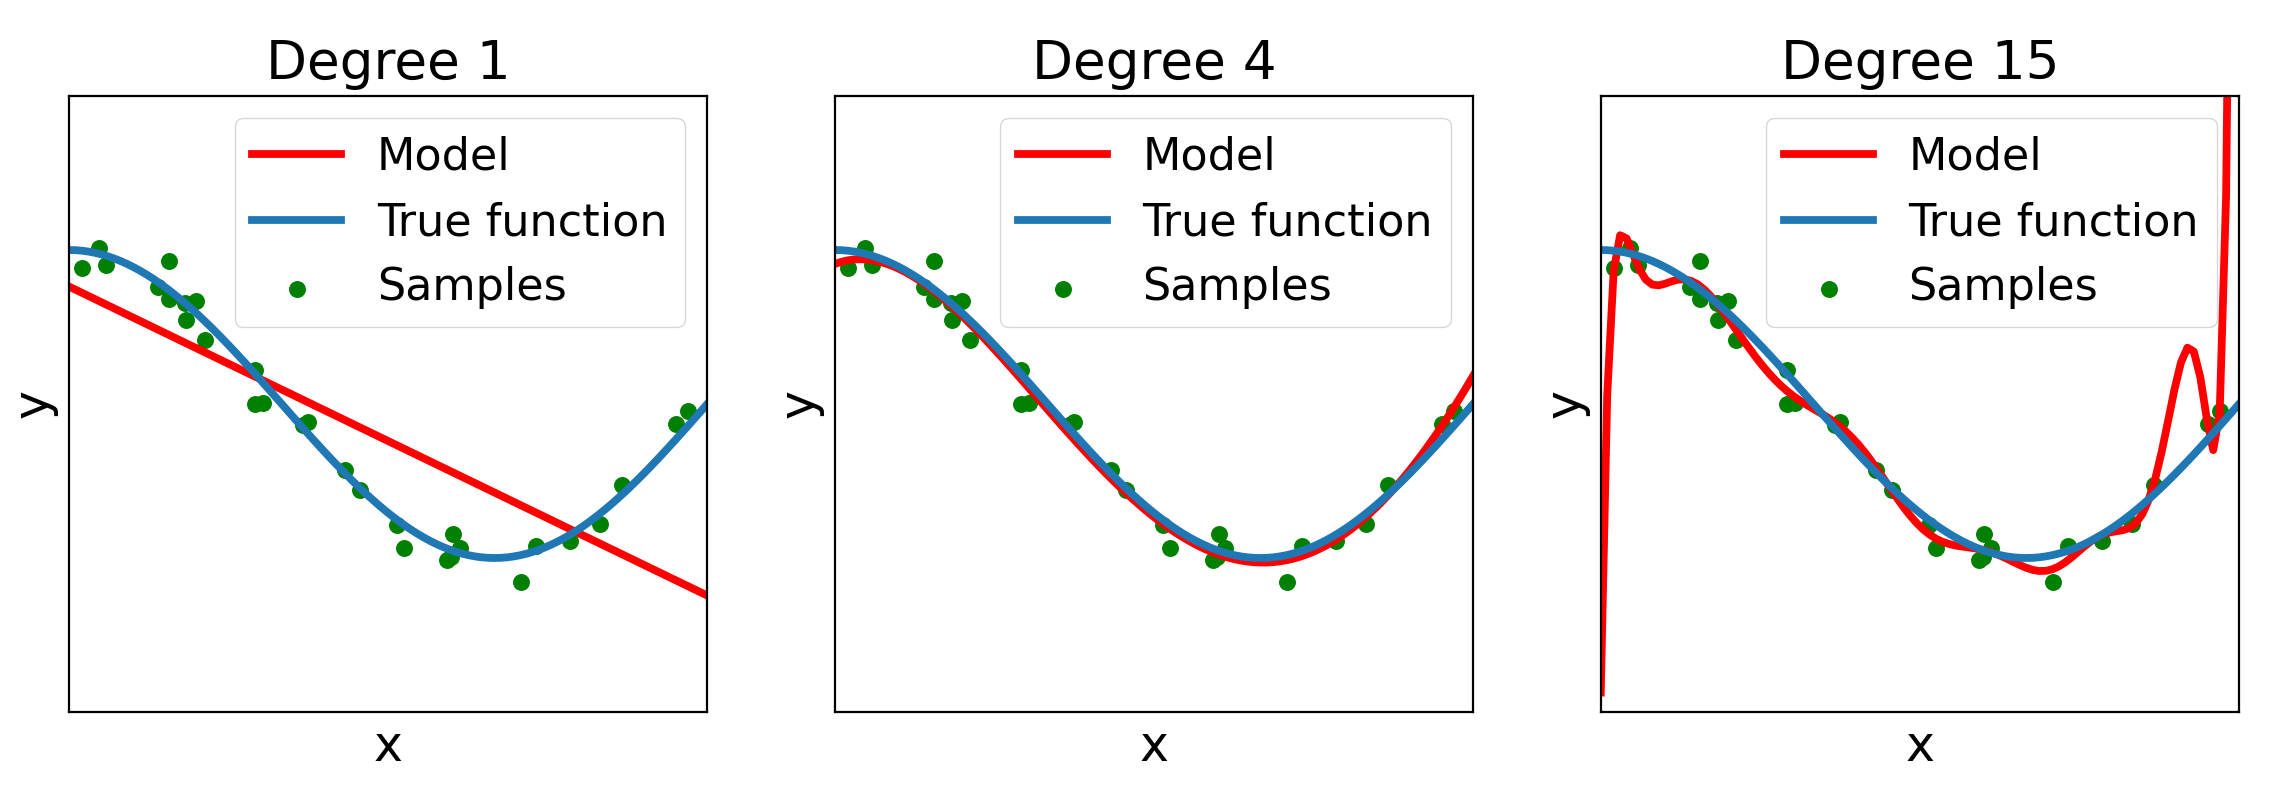
\includegraphics[scale=0.35]{images/overfitting_poly}
			\caption{Underfitting (degree 1), good fitting (degree 4), overfitting (degree 15).}
		\end{figure}
	\end{frame}

	\begin{frame}
		\frametitle{How to counter overfitting}
	\end{frame}
\end{document}